\documentclass[border=3mm]{standalone}

\usepackage{tikz}

\begin{document}
	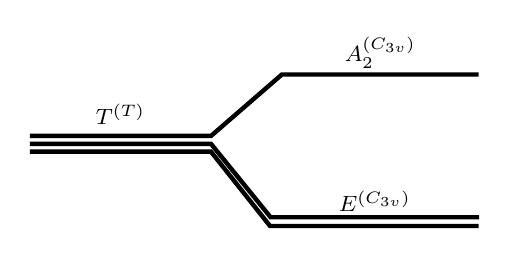
\begin{tikzpicture}
		\draw [ultra thick] (-2.9407,-0.1799) -- (-0.6407,-0.1799) node[above,midway] {\footnotesize $T^{(T)}$}-- (0.2593,0.6001) -- (2.7593,0.6001) node[above,midway,yshift=-2pt] {\footnotesize $A_2^{(C_{3v})}$};
		\draw [ultra thick] (-2.9407,-0.2799) -- (-0.6407,-0.2799) -- (0.116,-1.2123) -- (2.766,-1.2123) node[above,midway,yshift=-2pt] {\footnotesize $E^{(C_{3v})}$};
		\draw [ultra thick] (-2.9407,-0.3799) -- (-0.6407,-0.3799) -- (0.1093,-1.3236) -- (2.7593,-1.3236);
	\end{tikzpicture}
\end{document}